\chapter{强化学习}

现在开始学习强化学习和自适应控制。

监督学习中的算法试图使其输出模仿训练集中的标签 $y$。在这种设置下,对于每个输入 $x$,标签都给出了明确的“正确答案”。然而,对于许多序列决策和控制问题,很难为学习算法提供这种显式监督。例如,如果我们构建了一个四足机器人并试图对其进行编程以使其行走,那么我们其实不知道什么是使其行走的“正确”动作,因此也不知道如何为学习算法提供显式监督以供其模仿。

强化学习将转而为算法提供一个奖励函数,该函数指示学习智能体何时表现良好,何时表现不佳。在四足行走示例中,奖励函数可以对机器人向前移动给予正奖励,而对向后移动或摔倒给予负奖励。然后,学习算法的任务就是随着时间推移确定如何选择动作以获得高奖励。

强化学习已成功应用于各种领域,包括自主直升机飞行、机器人腿部运动、蜂窝网络路由、营销策略选择、工厂控制和高效网页索引。对强化学习的研究将从定义\textbf{马尔可夫决策过程 (Markov decision processess, MDP)} 开始,它提供了表述强化学习问题的一般化形式化框架。

\section{马尔可夫决策过程}

马尔可夫决策过程是一个元组 $(S, A, \{P_{s a}\}, \gamma, R)$,其中:
\begin{itemize}
    \item $S$ 是一个\textbf{状态 (states)} 集合。(例如,在自主直升机飞行中,$S$ 可以是直升机所有可能的位置和方向的集合。)
    \item $A$ 是一个\textbf{动作 (actions)} 集合。(例如,可以推动直升机控制杆的所有可能方向的集合。)
    \item $P_{sa}$ 是状态转移概率 (state transition probabilities)。对于每个状态 $s \in S$ 和动作 $a \in A$, $P_{sa}$ 是状态空间上的一个分布。稍后会详细介绍,但简而言之,$P_{sa}$ 给出了如果在状态 $s$ 采取动作 $a$ 后将转移到哪些状态的分布。
    \item $\gamma \in [0, 1]$ 称为\textbf{折扣因子 (discount factor)}。
    \item $R: S \times A \mapsto \mathbb{R}$ 是\textbf{奖励函数 (reward function)}。(奖励有时也写成仅关于状态 $S$ 的函数,在这种情况下有 $R: S \mapsto \mathbb{R}$)。
\end{itemize}
MDP 的动态过程如下:我们从某个状态 $s_0$ 开始,然后在 MDP 中选择一个动作 $a_0 \in A$ 执行。然后 MDP 的状态随机转移到某个后继状态 $s_1$,根据 $s_1 \sim P_{s_0 a_0}$ 抽取。然后选择另一个动作 $a_1$。由于这个动作,状态再次转移,现在转移到某个 $s_2 \sim P_{s_1 a_1}$,依此类推。可以将这个过程表示为:
\[
    s_0 \xrightarrow{a_0} s_1 \xrightarrow{a_1} s_2 \xrightarrow{a_2} s_3 \xrightarrow{a_3} \dots
\]

以动作序列 $a_0, a_1, \dots$ 遍历状态序列 $s_0, s_1, \dots$ 后,总收益由下式给出
\[
    R(s_0, a_0) + \gamma R(s_1, a_1) + \gamma^2 R(s_2, a_2) + \dots.
\]
或者,将奖励写成仅关于状态的函数时,则变为
\[
    R(s_0) + \gamma R(s_1) + \gamma^2 R(s_2) + \dots.
\]
在大部分推导中,将使用更简单的状态奖励 $R(s)$,尽管推广到状态-动作奖励 $R(s, a)$ 也不会有特别的困难。

在强化学习中,目标是随着时间推移选择动作以最大化总收益的期望值:
\[
    \text{E}\left[R(s_0) + \gamma R(s_1) + \gamma^2 R(s_2) + \dots\right]
\]
注意,时间步 $t$ 的奖励被 $\gamma^t$ \textbf{折扣 (discount)}。因此,为了使这个期望值最大化,希望尽快累积正奖励(并尽可能推迟负奖励)。在经济应用中,如果 $R(\cdot)$ 代表赚取的金额,那么 $\gamma$ 也有一个自然的利率解释(今天的一美元比明天的一美元更值钱)。

\textbf{策略 (policy)} 是一个函数 $\pi: S \mapsto A$,它将状态映射到动作。当处于状态 $s$ 时,如果\textbf{执行 (executing)} 某个策略 $\pi$,则采取动作 $a = \pi(s)$。同时定义策略 $\pi$ 的\textbf{价值函数 (value function)} 为
\[
    V^\pi(s) = \text{E}\left[R(s_0) + \gamma R(s_1) + \gamma^2 R(s_2) + \dots \mid s_0 = s, \pi\right].
\]
$V^\pi(s)$ 表示从状态 $s$ 开始并按照策略 $\pi$ 采取动作所获得的折扣奖励的期望总和。\footnote{请注意,这里以 $\pi$ 为条件的写法并不完全正确,因为 $\pi$ 不是随机变量,但这在文献中是相当标准的用法。}

给定一个固定的策略 $\pi$,其价值函数 $V^\pi$ 满足\textbf{贝尔曼方程 (Bellman equation)}:
\[
    V^\pi(s) = R(s) + \gamma \sum_{s' \in S} P_{s\pi(s)}(s') V^\pi(s').
\]
这表明从状态 $s$ 开始的折扣奖励期望总和 $V^\pi(s)$ 由两部分组成:第一部分是从状态 $s$ 开始即刻获得的\textbf{即时奖励 (immediate reward)} $R(s)$;第二部分是未来折扣奖励的期望总和。仔细考察第二项,可以看到上面的求和项可以重写为 $\text{E}_{s' \sim P_{s\pi(s)}}[V^\pi(s')]$。这是从状态 $s'$ 开始的折扣奖励的期望总和,其中 $s'$ 的分布由 $P_{s\pi(s)}$ 给出,也就是在 MDP 中从状态 $s$ 执行第一个动作 $\pi(s)$ 后将到达的状态分布。因此,上面的第二项给出的是在 MDP 中执行第一步后获得的折扣奖励的期望总和。

贝尔曼方程可以有效地用于求解 $V^\pi$。具体来说,在一个有限状态 MDP ($|S| < \infty$) 中,可以为每个状态 $s$ 写出一个关于 $V^\pi(s)$ 的方程。这给出了 $|S|$ 个线性方程组,其中包含 $|S|$ 个变量(未知的 $V^\pi(s)$),可以有效地求解这些变量。

同样地,定义\textbf{最优价值函数 (optimal value function)} 为
\begin{equation}
    V^*(s) = \max_{\pi} V^\pi(s).
    \label{eq:15.1}
\end{equation}
换句话说,这是使用任何策略可以达到的最佳期望折扣奖励总和。对于最优价值函数,也有一个贝尔曼方程:
\begin{equation}
    V^*(s) = R(s) + \max_{a \in A} \gamma \sum_{s' \in S} P_{sa}(s') V^*(s').
    \label{eq:15.2}
\end{equation}
上面的第一项是即时奖励。第二项是在执行动作 $a$ 之后获得的期望未来折扣奖励总和在所有动作 $a$ 上的最大值。应该确保理解这个方程及其合理性。

同时定义策略 $\pi^*: S \mapsto A$ 如下:
\begin{equation}
    \pi^*(s) = \arg \max_{a \in A} \sum_{s' \in S} P_{sa}(s') V^*(s').
    \label{eq:15.3}
\end{equation}
注意,$\pi^*(s)$ 给出了在方程\eqref{eq:15.2}中的 "max" 中达到最大值的动作 $a$。

事实证明,对于每一个状态 $s$ 和每一个策略 $\pi$,有
\[
    V^*(s) = V^{\pi^*}(s) \ge V^\pi(s).
\]
第一个等号表示,对于每个状态 $s$,策略 $\pi^*$ 的价值函数 $V^{\pi^*}$ 都等于最优价值函数 $V^*$。此外,不等号表示 $\pi^*$ 的价值至少与任何其他策略的价值一样大。换句话说,方程 \eqref{eq:15.3} 所定义的 $\pi^*$ 是\textbf{最优策略 (optimal policy)}。

注意,$\pi^*$ 具有一个有趣的性质,即它是\textit{所有 (all)} 状态 $s$ 的最优策略。也就是说,不会是这样:从某个状态 $s$ 开始的最优策略,与从另一个状态 $s'$ 开始的最优策略不同。同一个策略 $\pi^*$ 在\textit{所有 (all)} 状态 $s$ 下都达到了方程 \eqref{eq:15.1} 的最大值。这意味着无论 MDP 的初始状态是什么,都可以使用相同的策略 $\pi^*$。

\section{价值迭代与策略迭代}\label{sec:15.2}

现在介绍两种求解有限状态 MDP 的高效算法。目前,只考虑具有有限状态空间和动作空间(即 $|S| < \infty, |A| < \infty$)的 MDP。在本节中,还假设已知状态转移概率 $\{P_{sa}\}$ 和奖励函数 $R$。

第一个算法是\textbf{价值迭代 (value iteration)},如下所示:

\vspace{0.5em}
\begin{algorithm}[H]
    \SetAlgoNoLine
    \label{algo:4}
    \caption{价值迭代}
    对于每个状态 $s$,初始化 $V(s) := 0$。\\
    \For{直到收敛}{
        对于每个状态,更新
        \begin{equation}\label{eq:15.4}
            V(s) := R(s) + \max_{a \in A} \gamma \sum_{s'} P_{sa}(s') V(s').
        \end{equation}
    }
\end{algorithm}

这个算法可以看作是重复使用贝尔曼方程\eqref{eq:15.2}来更新估计的价值函数。

算法的内循环中更新 $V(s)$ 的方式有两种方式。第一种是先计算每个状态 $s$ 的新 $V(s)$ 值,然后用新值覆盖所有旧值。这称为\textbf{同步 (synchronous)} 更新。在这种情况下,算法可以看作是实现了一个“贝尔曼备份算子”,它接收价值函数的当前估计,并将其映射到一个新的估计。(详请参阅习题集。)另一种方法是执行\textbf{异步 (asynchronous)} 更新。在这种情况下,可以按某种顺序逐个状态进行循环,每次更新一个值。

在同步或异步更新下,可以证明价值迭代会使 $V$ 收敛到 $V^*$。找到 $V^*$ 后,可以使用方程\eqref{eq:15.3}来找到最优策略。

除了价值迭代,还有另一种算法用于寻找 MDP 的最优策略。\textbf{策略迭代 (policy iteration)} 算法如下:

\vspace{0.5em}
\begin{algorithm}[H]
    \SetKwComment{Comment}{$\triangleright$\ }{}
    \SetAlgoNoLine
    \label{algo:5}
    \caption{策略迭代}
    随机初始化 $\pi$。\\
    \For{直到收敛}{
        令 $V := V^\pi.$ \Comment*[f]{通常用线性系统求解器处理}\\
        对于每个状态 $s$,令
        \begin{equation*}
            \pi(s) := \arg\max_{a \in A} \sum_{s'}P_{s a}(s')V(s').
        \end{equation*}
    }
\end{algorithm}

因此,内循环重复计算当前策略的价值函数,然后使用当前价值函数更新策略。(步骤 (b) 中找到的策略也称为关于 $V$ 的\textbf{贪婪策略 (greedy policy)}。)注意,步骤 (a) 可以通过求解贝尔曼方程来实现,如前所述,对于一个固定的策略,这仅仅是关于 $|S|$ 个变量的 $|S|$ 个线性方程组。
经过该算法的\textit{有限 (finite)} 次迭代后,$V$ 将收敛到 $V^*$,并且 $\pi$ 将收敛到 $\pi^*$。\footnote{注意,价值迭代无法在有限次迭代中达到精确的 $V^*$,但策略迭代可以使用精确的线性方程组求解器,因此可以精确收敛。这是因为当动作空间和策略空间是离散且有限时,一旦策略迭代中的策略达到最优策略,它将不再改变。另一方面,尽管价值迭代会收敛到 $V^*$,但学习到的价值函数中总是存在一些非零误差。}

价值迭代和策略迭代都是求解 MDP 的标准算法,目前对于哪种算法更好还没有普遍共识。对于小型 MDP,策略迭代通常非常快,并且在很少的迭代次数内收敛。然而,对于状态空间较大的 MDP,显式求解 $V^*$ 将涉及求解一个大型线性方程组,这可能会很困难(并且注意在策略迭代中需要多次求解线性方程组)。在这些问题中,价值迭代可能更受欢迎。因此,在实践中,价值迭代似乎比策略迭代更常用。关于价值迭代和策略迭代的比较和联系的更多讨论,请参阅第 \ref{sec:15.5} 节。

\section{学习 MDP 的模型}

到目前为止,所讨论的 MDP 和求解 MDP 的算法都假设已知状态转移概率和奖励。在许多现实问题中,我们无法直接获得状态转移概率和奖励,而是必须从数据中估计它们。(通常,状态空间 $S$、动作空间 $A$ 和折扣因子 $\gamma$ 是已知的。)例如,假设对于倒立摆问题(参见习题集 4),我们在 MDP 中进行了一些试验,过程如下:
\begin{align*}
    &s_0^{(1)} \xrightarrow{a_0^{(1)}} s_1^{(1)} \xrightarrow{a_1^{(1)}} s_2^{(1)} \xrightarrow{a_2^{(1)}} s_3^{(1)} \xrightarrow{a_3^{(1)}} \dots \\
    &s_0^{(2)} \xrightarrow{a_0^{(2)}} s_1^{(2)} \xrightarrow{a_1^{(2)}} s_2^{(2)} \xrightarrow{a_2^{(2)}} s_3^{(2)} \xrightarrow{a_3^{(2)}} \dots\\
    &\cdots
\end{align*}
这里,$s_i^{(j)}$ 是在第 $j$ 次试验的时刻 $i$ 时的状态,$a_i^{(j)}$ 是在该状态下采取的相应动作。在实践中,上述每一次试验可能会持续到 MDP 终止(例如,倒立摆问题中,摆杆倒下),或者可能运行很长但有限的时间步。

给定由多次试验组成的 MDP 中的这种“经验”,可以很容易地得出状态转移概率的最大似然估计:
\begin{equation}
    P_{sa}(s') = \frac{\text{在状态 $s$ 采取动作 $a$ 到达状态 $s'$ 的次数}}{\text{在状态 $s$ 采取动作 $a$ 的次数}}
    \label{eq:15.5}
\end{equation}
或者,如果上述比率是“0/0”——对应于之前从未在状态 $s$ 采取动作 $a$ 的情况——我们可以简单地将 $P_{sa}(s')$ 估计为 $1/|S|$。(即,将 $P_{sa}$ 估计为关于所有状态的均匀分布。)

注意,如果得到了更多经验(观察了更多试验),有一种有效的方法可以使用新的经验更新状态转移概率估计。具体来说,如果我们跟踪 \eqref{eq:15.5} 中分子和分母的计数,那么当观察更多试验时,可以简单地累加这些计数。计算这些计数的比率即可得到对 $P_{sa}$ 的估计。

使用类似的过程,如果 $R$ 未知,也可以将状态 $s$ 中预期即时奖励 $R(s)$ 的估计值取为在状态 $s$ 中观察到的平均奖励。

在学习了 MDP 的模型后,可以使用价值迭代或策略迭代来求解 MDP,使用估计的状态转移概率和奖励。例如,将模型学习和价值迭代结合起来,是学习具有未知状态转移概率的 MDP 的一种可能的算法:

\begin{enumerate}
    \item 随机初始化 $\pi$。
    \item 重复 \{
        \begin{enumerate}
            \item 在 MDP 中执行一定次数的 $\pi$,收集经验。
            \item 使用上述经验更新状态转移概率 $P_{sa}$ 的估计值(如果可行的话,也更新 $R$ 的估计值)。
            \item 根据估计的状态转移概率和奖励,使用价值迭代更新价值函数 $V$ 的估计值。
            \item 更新策略 $\pi$,使其成为关于 $V$ 的贪婪策略。
        \end{enumerate}
    \}
\end{enumerate}

注意到,对于该算法,有一个简单的优化可以使其运行得更快。具体来说,在算法的内层循环中,应用价值迭代时,如果不是将价值迭代初始化为 $V=0$,而是用算法前一次迭代中找到的解进行初始化,那么这将为价值迭代提供一个更好的起始点,并使其更快收敛。

\section{连续状态 MDP}

之前我们主要关注了有限状态数量的 MDP。现在我们将讨论可能具有无限状态数量的 MDP 的算法。例如,对于汽车,我们可以将状态表示为 $(x, y, \theta, \dot{x}, \dot{y}, \dot{\theta})$,其中包括其位置 $(x, y)$;方向 $\theta$;在 $x$ 和 $y$ 方向上的速度 $\dot{x}$ 和 $\dot{y}$;以及角速度 $\dot{\theta}$。因此,$S = \mathbb{R}^6$ 是一个无限状态集,因为汽车有无限多的可能位置和方向。\footnote{严格来说,$\theta$ 是一个方向,因此 $\theta$ 的范围写成 $\theta \in [-\pi, \pi)$ 比 $\theta \in \mathbb{R}$ 更合适;但对我们的目标而言,这种区别并不重要。} 类似地,在习题集 4 中的倒立摆具有状态 $(x, \theta, \dot{x}, \dot{\theta})$,其中 $\theta$ 是摆杆的角度。而一架在 3D 空间中飞行的直升机具有 $(x, y, z, \phi, \theta, \psi, \dot{x}, \dot{y}, \dot{z}, \dot{\phi}, \dot{\theta}, \dot{\psi})$ 形式的状态,其中横滚角 $\phi$、俯仰角 $\theta$ 和偏航角 $\psi$ 指定了直升机的 3D 方向。

在本节中,我们将考虑状态空间为 $S = \mathbb{R}^d$ 的情况,并描述解决此类 MDP 的方法。

\subsection{离散化}

解决连续状态 MDP 的最简单方法可能是离散化状态空间,然后使用之前描述的价值迭代或策略迭代等算法。

例如,对于 2D 状态 $(s_1, s_2)$,可以使用网格来离散化状态空间:

\begin{figure}[H]
    \centering
    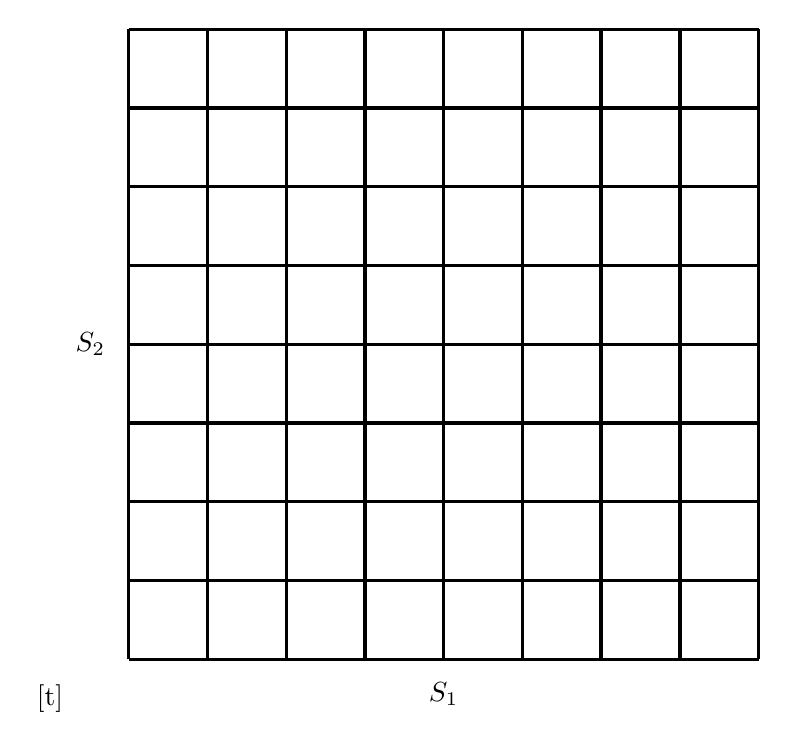
\begin{tikzpicture}
        \def\gridsize{8}
        \draw[step=1, very thick, black] (0,0) grid (\gridsize, \gridsize);
        \node[below=5pt] at (\gridsize/2, 0) {$S_1$};
        \node[left=5pt] at (0, \gridsize/2) {$S_2$};
        \node at (-1, -0.5) {[t]};
    \end{tikzpicture}
\end{figure}

这里,每个网格单元代表一个独立的离散状态 $\bar{s}$。然后,可以通过一个离散状态 MDP $(\bar{S}, A, \{P_{\bar{s}a}\}, \gamma, R)$ 来近似连续状态 MDP,其中 $\bar{S}$ 是离散状态的集合,$\{P_{\bar{s}a}\}$ 是离散状态上的状态转移概率。然后,可以使用价值迭代或策略迭代来解出离散状态 MDP $(\bar{S}, A, \{P_{\bar{s}a}\}, \gamma, R)$ 中的 $V^*(\bar{s})$ 和 $\pi^*(\bar{s})$。当实际系统处于某个连续值状态 $s \in S$ 并且需要选择一个动作来执行时,就计算相应的离散化状态 $\bar{s}$,并执行动作 $\pi^*(\bar{s})$。

这种离散化方法对于许多问题都能很好地工作。然而,它有两个缺点。首先,它对 $V^*$(以及 $\pi^*$)使用了相当简单的表示。具体来说,它假设价值函数在每个离散化区间上取一个常数值(即,价值函数在每个网格单元中是分段常数)。

为了更好地理解这种表示的局限性,考虑一个\textit{监督学习 (supervised learning)} 问题,将函数拟合到这个数据集:

\begin{figure}[H]
    \centering
    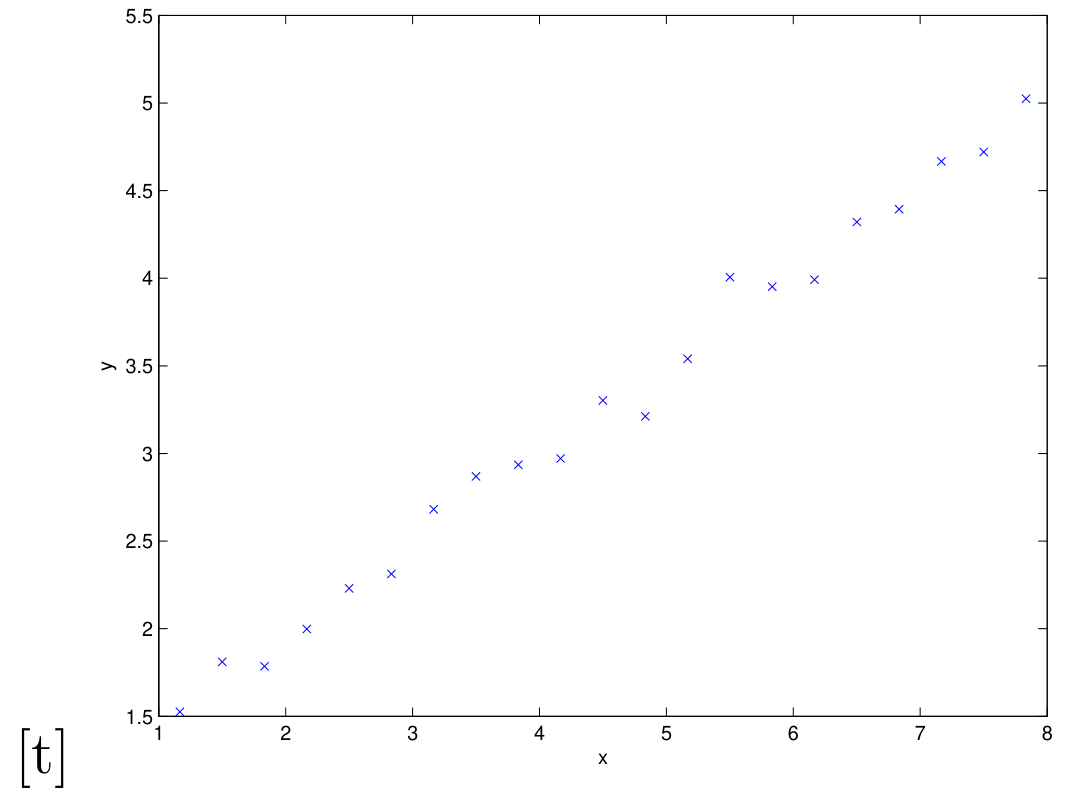
\includegraphics[width=0.6\textwidth]{figs/rl_dataset.png}
\end{figure}

显然,线性回归可以很好地拟合这个数据集,然而,如果对 x 轴离散化,并使用在每个离散区间内为分段常数的表示,那么我们对数据的拟合将如下所示:

\begin{figure}[H]
    \centering
    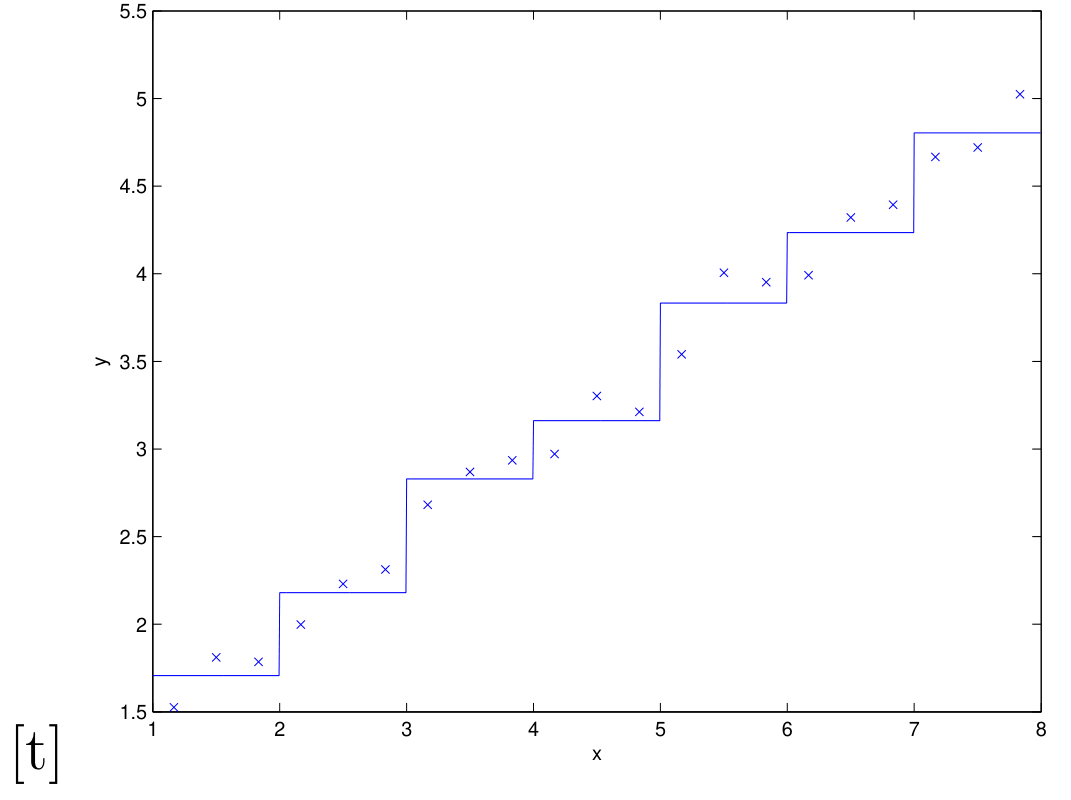
\includegraphics[width=0.6\textwidth]{figs/rl_dataset_discrete.png}
\end{figure}

这种分段常数表示对于许多平滑函数来说并不是一个好的表示。它导致输入上的平滑性很差,并且在不同网格单元之间没有泛化能力。使用这种表示,我们需要非常精细的离散化(非常小的网格单元)才能获得良好的近似。

这种表示的第二个缺点被称为\textbf{维度诅咒 (curse of dimensionality)}。假设 $S = \mathbb{R}^d$,并且我们将状态的 $d$ 个维度中的每一个都离散化为 $k$ 个值。那么我们拥有的离散状态总数为 $k^d$。这在状态空间维度 $d$ 中呈指数级增长,因此不适用于大型问题。例如,对于一个 10 维状态,如果我们将每个状态变量离散化为 100 个值,我们将有 $100^{10} = 10^{20}$ 个离散状态,这对于现代计算机来说也大到无法表示。

根据经验,离散化通常对于 1 维和 2 维问题非常有效(而且简单且快速实现)。也许用一些取巧的办法,并在选择离散化方法时谨慎一些,它也能适用于 4 维状态的问题。如果你非常聪明且幸运,甚至可能让它适用于某些 6 维问题。但它很少适用于更高维度的问题。

\subsection{价值函数近似}

我们现在介绍一种在连续状态 MDP 中寻找策略的替代方法,即直接近似 $V^*$,而无需诉诸离散化。这种方法被称为价值函数近似,且已成功应用于许多强化学习问题。

\subsubsection*{使用模型或模拟器}

为了开发值函数近似算法,我们将假设我们拥有一个用于 MDP 的\textbf{模型 (model)} 或\textbf{模拟器 (simulator)}。非正式地,模拟器是一个黑盒,它接收任何(连续值)状态 $s_t$ 和动作 $a_t$ 作为输入,并根据状态转移概率 $P_{s_t a_t}$ 输出下一个状态 $s_{t+1}$ 的采样。

\begin{figure}[H]
    \centering
    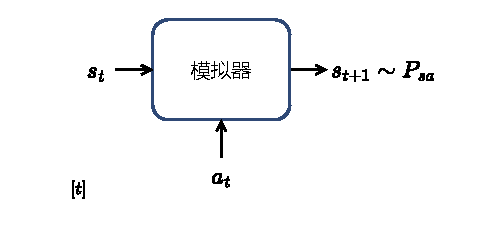
\includegraphics[width=0.5\textwidth]{figs/simulator.pdf}
\end{figure}

获取此类模型有多种方法。一种是使用物理模拟。例如,习题集 4 中倒立摆的模拟器是通过使用物理定律计算在给定当前状态 $t$ 和所采取的动作 $a$ 的情况下,小车/杆在时间 $t+1$ 的位置和方向来获得的,前提是已知系统的所有参数,例如杆的长度、杆的质量等。或者,也可以使用现成的物理模拟软件包,该软件包将机械系统的完整物理描述、当前状态 $s_t$ 和动作 $a_t$ 作为输入,并在未来一小段时间内计算出系统的状态 $s_{t+1}$。\footnote{Open Dynamics Engine (\url{http://www.ode.com}) 是一个免费/开源的物理模拟器示例,可用于模拟倒立摆等系统,并且在强化学习研究人员中一直是一个受欢迎的选择。}

获取模型的另一种方法是从 MDP 中收集的数据中学习一个模型。例如,假设执行 $n$ 次\textbf{试验 (trials)},每次试验重复在 MDP 中采取动作,且持续 $T$ 个时间步。可以随机选择动作、执行某些特定策略或通过其他方式选择动作。然后,将观察到 $n$ 个状态序列,如下所示:
\begin{align*}
    &s_0^{(1)} \xrightarrow{a_0^{(1)}} s_1^{(1)} \xrightarrow{a_1^{(1)}} s_2^{(1)} \xrightarrow{a_2^{(1)}} \dots \xrightarrow{a_{T-1}^{(1)}} s_T^{(1)} \\
    &s_0^{(2)} \xrightarrow{a_0^{(2)}} s_1^{(2)} \xrightarrow{a_1^{(2)}} s_2^{(2)} \xrightarrow{a_2^{(2)}} \dots \xrightarrow{a_{T-1}^{(2)}} s_T^{(2)} \\
    &\dots \\
    &s_0^{(n)} \xrightarrow{a_0^{(n)}} s_1^{(n)} \xrightarrow{a_1^{(n)}} s_2^{(n)} \xrightarrow{a_2^{(n)}} \dots \xrightarrow{a_{T-1}^{(n)}} s_T^{(n)}
\end{align*}
然后,可以应用学习算法来预测 $s_{t+1}$ 作为 $s_t$ 和 $a_t$ 的函数。

例如,可以选择学习一个如下形式的线性模型:
\begin{equation}
    s_{t+1} = As_t + Ba_t,
    \label{eq:15.6}
\end{equation}
使用类似于线性回归的算法。这里,模型的参数是矩阵 $A$ 和 $B$,并且可以通过从 $n$ 次试验中收集的数据来估计它们:
\[
    \underset{A,B}{\arg \min} \sum_{i=1}^n \sum_{t=0}^{T-1} \left\| s_{t+1}^{(i)} - (As_t^{(i)} + Ba_t^{(i)}) \right\|^2.
\]

也可以使用其他损失函数来学习模型。例如,最近 \cite{luo2018algorithmic} 的工作发现,使用 $\left\| \cdot \right\|_2$ 范数(不带平方)在某些情况下可能有所帮助。

在学习了 $A$ 和 $B$ 之后,一个选项是构建一个\textbf{确定性 (deterministic)} 模型,其中给定输入 $s_t$ 和 $a_t$,输出 $s_{t+1}$ 被精确确定。具体来说,总是根据公式 \eqref{eq:15.6} 计算 $s_{t+1}$。或者,也可以构建一个\textbf{随机 (stochastic)} 模型,其中 $s_{t+1}$ 是输入的随机函数,通过将其建模为:
\[
    s_{t+1} = As_t + Ba_t + \epsilon_t,
\]
其中 $\epsilon_t$ 是一个噪声项,通常建模为 $\epsilon_t \sim \mathcal{N}(0, \Sigma)$。(协方差矩阵 $\Sigma$ 也可以以直接的方式从数据中估计。)

这里将下一个状态 $s_{t+1}$ 写成当前状态和动作的线性函数;当然,这也可以是非线性函数。具体来说,可以学习一个模型 $s_{t+1} = A\phi_s(s_t) + B\phi_a(a_t)$,其中 $\phi_s$ 和 $\phi_a$ 是状态和动作的一些非线性特征映射。或者,也可以使用非线性学习算法,例如局部加权线性回归,来估计 $s_{t+1}$ 作为 $s_t$ 和 $a_t$ 的函数。这些方法都可以用来构建 MDP 的确定性或随机模拟器。

\subsubsection*{拟合价值迭代}

现在介绍用于近似连续状态 MDP 价值函数的\textbf{拟合价值迭代 (fitted value iteration)} 算法。在下文中,我们将假设问题具有连续状态空间 $S = \mathbb{R}^d$,但动作空间 $A$ 较小且离散。\footnote{在实践中,大多数 MDP 的动作空间远小于状态空间。例如,汽车状态空间有 6 维而动作空间则是 2 维(转向和速度控制);倒立摆状态空间有 4 维而动作空间只有 1 维;直升机则是 12 维状态空间和 4 维动作空间。因此,离散化动作空间通常比离散化状态空间的问题要小得多。}

回顾一下,价值迭代执行以下更新:
\begin{align}
    V(s) &:= R(s) + \gamma \max_a \int_{s'} P_{sa}(s')V(s')ds' \label{eq:15.7} \\
    &= R(s) + \gamma \max_a \mathrm{E}_{s' \sim P_{sa}} [V(s')] \label{eq:15.8}
\end{align}
(在第 \ref{sec:15.2} 节中,价值迭代更新写为 $V(s) := R(s) + \gamma \max_a \sum_{s'} P_{sa}(s')V(s')$ 而不是状态上的积分;新的符号反映了现在正在处理连续状态而不是离散状态。)

拟合价值迭代的主要思想是,在有限样本状态 $s^{(1)}, \dots, s^{(n)}$ 上近似地执行此步骤。具体来说,下面使用监督学习算法——线性回归——来近似状态的价值函数,作为状态的线性或非线性函数:
\[
    V(s) = \theta^T \phi(s).
\]
这里,$\phi$ 是状态的某种适当的特征映射。

对于具有的有限样本 $n$ 个状态中的每个状态 $s$,拟合价值迭代将首先计算一个量 $y^{(i)}$,是 $R(s) + \gamma \max_a \mathrm{E}_{s' \sim P_{sa}} [V(s')]$ 的近似(公式 \eqref{eq:15.8} 的右侧)。然后将应用监督学习算法,尝试使 $V(s)$ 接近 $R(s) + \gamma \max_a \mathrm{E}_{s' \sim P_{sa}} [V(s')]$(换句话说,尝试使 $V(s)$ 接近 $y^{(i)}$)。

详细来说,该算法如下:
\begin{enumerate}
    \item 随机采样 $n$ 个状态 $s^{(1)}, s^{(2)}, \cdots, s^{(n)} \in S$。
    \item 初始化 $\theta := 0$。
    \item 重复 \{
        \begin{itemize}
            \item[] 对于 $i = 1, \dots, n$ \{
                \begin{itemize}
                    \item[] 对于每个动作 $a \in A$ \{
                        \begin{itemize}
                            \item[] 采样 $s_1', \cdots, s_k' \sim P_{s^{(i)} a}$(使用某种 MDP 模型)。
                            \item[] 令 $q(a)=\frac1k \sum_{j=1}^{k} R(s^{(i)}) + \gamma V(s_j')$。
                            \item[] \qquad // 因此,$q(a)$ 是 $R(s^{i}) + \gamma \mathrm{E}_{s'\sim P_{s^{(i) a}}}[V(s')]$ 的估计值。
                        \end{itemize}

                    \}
                    \item[] 令 $y^{(i)} = \max_a q(a)$。
                    \item[] \qquad // 因此, $y^{(i)}$ 是 $R(s^{i}) + \gamma \max_a \mathrm{E}_{s'\sim P_{s^{(i) a}}}[V(s')]$ 的估计值。
                \end{itemize}
            \}
            \item[] // 原始的(用于离散状态的)价值迭代算法
            \item[] // 根据 $V(s^{(i)}) := y^{(i)}$ 更新价值函数。
            \item[] // 此算法则希望 $V(s^{(i)}) \approx y^{(i)}$
            \item[] // 可以使用监督学习(线性回归)达成这点。
            \item[] 令 $\theta := \arg\min_\theta \frac12 \sum_{i=1}^{n} \left(\theta^T \phi(s^{(i)}) - y^{(i)}\right)^2$。
        \end{itemize}
        
    \}
\end{enumerate}

如上所述,我们已经详细阐述了使用线性回归的拟合价值迭代算法,以使 $V(s^{(i)})$ 接近 $y^{(i)}$。算法的这一步骤完全类似于标准的监督学习(回归)问题,其中有一个训练集 $(x^{(1)}, y^{(1)}), (x^{(2)}, y^{(2)}), \dots, (x^{(n)}, y^{(n)})$,并且希望学习一个从 $x$ 到 $y$ 的函数;唯一的区别是这里 $s$ 扮演了 $x$ 的角色。尽管上面的描述使用了线性回归,但显然也可以使用其他回归算法(例如局部加权线性回归)。

与离散状态集上的价值迭代不同,拟合价值迭代不能被证明总是收敛的。然而,它在实践中通常能收敛(或近似收敛),并且对许多问题都表现良好。还需要注意的是,如果使用 MDP 的确定性模拟器/模型,那么可以通过在算法中设置 $k=1$ 来简化拟合价值迭代。这是因为公式 \eqref{eq:15.8} 中的期望变为确定性分布上的期望,因此一个单一的样本就足以精确计算该期望。否则,在上述算法中,需要抽取 $k$ 个样本并取平均值来近似该期望(参见算法伪代码中 $q(a)$ 的定义)。

最后,拟合价值迭代输出 $V$ 作为 $V^*$ 的近似。这隐式地定义了我们的策略。具体来说,当系统处于某个状态 $s$,需要选择一个动作时,我们希望选择以下动作:
\begin{equation}
    \arg \max_a \mathrm{E}_{s' \sim P_{sa}} [V(s')] \label{eq:15.9}
\end{equation}
计算/近似此过程类似于拟合价值迭代的内循环,其中对于每个动作,我们从 $P_{sa}$ 中采样 $s'_1, \dots, s'_k$ 来近似期望。(同样,如果模拟器是确定性的,我们可以设置 $k=1$。)

在实践中,通常还有其他方法来近似此步骤。例如,一个非常常见的情况是模拟器具有 $s_{t+1} = f(s_t, a_t) + \epsilon_t$ 的形式,其中 $f$ 是状态的某个确定性函数(例如 $f(s_t, a_t) = As_t + Ba_t$),$\epsilon_t$ 是零均值高斯噪声。在这种情况下,我们可以通过以下方式选择动作:
\[
    \arg \max_a V(f(s, a)).
\]
换句话说,这里是设置 $\epsilon_t = 0$(即,忽略模拟器中的噪声),并设置 $k=1$。等效地,这可以从公式 \eqref{eq:15.9} 使用以下近似导出:
\begin{align}
    \mathrm{E}_{s'}[V(s')] &\approx V(\mathrm{E}_{s'}[s']) \label{eq:15.10} \\
    &= V(f(s, a)), \label{eq:15.11}
\end{align}
其中期望是关于随机变量 $s' \sim P_{sa}$ 的。只要噪声项 $\epsilon_t$ 很小,这通常是一个合理的近似。

然而,对于那些不适合这种近似的问题,为了近似上述期望,需要使用模型对 $k|A|$ 个状态进行采样,这在计算上可能非常昂贵。

\section{策略与价值的联系 (选读)}\label{sec:15.5}

\vspace{0.5em}
\begin{algorithm}[H]
    \SetKwComment{Comment}{$\triangleright$\ }{}
    \SetAlgoNoLine
    \label{algo:6}
    \caption{策略迭代的变体}
    \textbf{过程} VE($\pi$, k) \Comment*[f]{用于评估 $V^\pi$}\\
    \quad 选项 1:初始化 $V := 0$;选项 2:使用主算法的当前 $V$ 进行初始化。\\
    \quad \For{$i=0$ \KwTo $k-1$}{
        \quad 对于每个状态 $s$,更新
        \begin{equation}
            V(s) := R(s) + \gamma \sum_{s'} P_{s \pi(s)}(s')V(s').\label{eq:15.12}
        \end{equation}
    }
    \textbf{返回} $V$

    \ \\
    \textbf{输入}\ 超参数 $k$。\\
    随机初始化 $\pi$。\\
    \For{直到收敛}{
        令 $V := VE(\pi, k).$\\
        对于每个状态 $s$,令
        \begin{equation}
            \pi(s) := \arg\max_{a \in A} \sum_{s'}P_{s a}(s')V(s').\label{eq:15.13}
        \end{equation}
    }
\end{algorithm}

在策略迭代算法 \ref{algo:5} 的第 3 行,通常用线性系统求解器来计算 $V^\pi$。或者也可以使用迭代贝尔曼更新来评估 $V^\pi$,这类似于价值迭代,如算法 \ref{algo:6} 中过程 VE($\cdot$) 的第 1 行所示。如果我们在过程 VE 的第 2 行中选择选项 1,那么过程 VE 与价值迭代(算法 \ref{algo:4})的不同之处在其第 4 行:过程 VE 用 $\pi$ 中的动作,而价值迭代则使用贪婪动作。

用过程 VE 可以构建算法 \ref{algo:6},它是策略迭代的一种变体,作为连接策略迭代和价值迭代的中间算法。这里我们在 VE 中选用选项 2,以最大化重用之前所学的知识。可以验证,如果取 $k=1$ 并在算法 \ref{algo:6} 的第 2 行中选用选项 2,那么算法 \ref{algo:6} 在语义上等同于价值迭代(算法 \ref{algo:4})。换句话说,算法 \ref{algo:6} 和价值迭代交错更新 \eqref{eq:15.13} 和 \eqref{eq:15.12}。算法 \ref{algo:6} 在更新 $k$ 步 \eqref{eq:15.12} 和一步 \eqref{eq:15.13} 之间交替,而价值迭代在更新一步 \eqref{eq:15.12} 和一步 \eqref{eq:15.13} 之间交替。因此,算法 \ref{algo:6} 通常不会比价值迭代更快,因为假设更新 \eqref{eq:15.12} 和 \eqref{eq:15.13} 效用和耗时相同,那么更新频率的最佳平衡可能只是 $k=1$ 或 $k \approx 1$。

另一方面,如果更新 $k$ 步 \eqref{eq:15.12} 可以比更新一步 \eqref{eq:15.12} $k$ 次快得多,那么多求几步 \eqref{eq:15.12} 可能有用。这就是策略迭代所利用的——线性系统求解器求解 $k=\infty$ 的 VE 比求解较大的 $k$ 的 VE 会快得多。反之,如果不存在这种加速效果,例如当状态空间很大且线性系统求解器也不快时,价值迭代更可取。